\section{Exercise seven}

Consider the following code: 
\begin{verbatim}
I1: LD F6 32+ R2
I2: ADDD F2 F6 F4
I3: MULTD F0 F4 F2
I4: SUBD F12 F2 F6
I5: ADDD F0 F12 F2
\end{verbatim}
We have: 
\begin{itemize}
    \item 2 RESERVATION STATIONS (RS1, RS2) + 1 LOAD/STORE unit (LDU1) with latency 2
    \item 3 RESERVATION STATIONS (RS3, RS4, RS5) + 3 ALU/BR FUs (ALU1, ALU2, ALU3)    with latency 3
\end{itemize}
\begin{enumerate}
    \item Find all the conflicts. 
    \item Apply the Tomasulo algorithm. 
\end{enumerate}

\subsection*{Solution}
\begin{enumerate}
    \item The conflicts are the following: 
        \begin{itemize}
            \item RAW F6 I1-I2
            \item RAW F2 I2-I3
            \item RAW F2 I2-I4
            \item RAW F6 I1-I4
            \item RAW F2 I2-I5
            \item WAW F0 I3-I5
            \item RAW F12 I4-I5
        \end{itemize}
    \item The final result of the Tomasulo algorithm is: 
        \begin{figure}[H]
            \centering
            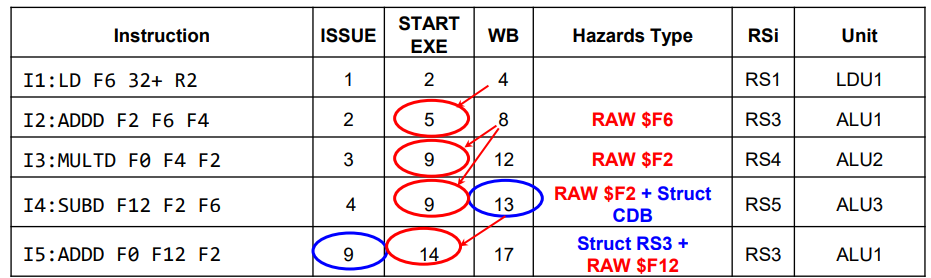
\includegraphics[width=1\linewidth]{images/tom.png}
        \end{figure}
\end{enumerate}